\documentclass[10pt] {article}

\usepackage[utf8]{inputenc}
\pagenumbering{arabic}
\usepackage{mathrsfs}
\usepackage[centertags]{amsmath}
\usepackage[usenames]{color}
\usepackage{mathrsfs}
\usepackage{newlfont}
\usepackage{enumerate}
\usepackage{graphicx}
\usepackage{multicol}
\usepackage[english]{babel}
\usepackage{natbib}
\usepackage{graphicx}
\usepackage{amssymb}
\usepackage{setspace} % for the line spacing
\usepackage{url}
\usepackage{imakeidx}
\usepackage{multicol}
\usepackage{float}
\usepackage{subfig}


\newcommand{\be}{\begin{equation}}
\newcommand{\ee}{\end{equation}}
\newcommand{\bean}{\begin{eqnarray}}
\newcommand{\eean}{\end{eqnarray}}
\newcommand{\bea}{\begin{eqnarray*}}
\newcommand{\eea}{\end{eqnarray*}}
\newcommand{\bfig}{\begin{figure}}
\newcommand{\efig}{\end{figure}}
\newcommand{\ba}{\begin{array}}
\newcommand{\ea}{\end{array}}
\newcommand{\na}{\nabla}
\newcommand{\pa}{\partial}
\newcommand{\Ra}{\Rightarrow \mbox{\hspace{1ex}}}
\newcommand{\ti}{\tilde}
\newcommand{\si}{\sigma}
\newcommand{\vsi}{\varsigma}
\newcommand{\ov}{\overline}
\newcommand{\ga}{\gamma}
\newcommand{\Ga}{\Gamma}
\newcommand{\eps}{\epsilon}
\newcommand{\ups}{\upsilon}
\newcommand{\Ups}{\Upsilon}
\newcommand{\var}{\varepsilon}
\newcommand{\ka}{\kappa}
\newcommand{\al}{\alpha}
\newcommand{\la}{\lambda}
\newcommand{\La}{\Lambda}
\newcommand{\de}{\delta}
\newcommand{\De}{\Delta}
\newcommand{\p}{\prime}
\newcommand{\ra}{\rightarrow}
\newcommand{\om}{\omega}
\newcommand{\Om}{\Omega}
\newcommand{\tha}{\theta}
\newcommand{\ze}{\zeta}
\newcommand{\bet}{\beta}
\newcommand{\et}{\eta}
\newcommand{\bs}{\boldsymbol}
\usepackage{hyperref}

\newtheorem{prev}{Remark}[section]

\parskip=6pt %para el espacio entre renglones
\hyphenrules{nohyphenation} %para que no rompa las palabras
\pretolerance=2000 \tolerance=3000

\singlespacing %\onehalfspacing,  \onehalfspacing, or \doublespacing, depending on the spacing you want

\newcommand\mord{{\raise1ex\hbox{\underbar{\scriptsize o}}}}
\newcommand\ford{\raise1ex\hbox{\underbar{\scriptsize a}}}

\usepackage{color}
\definecolor{Red}{rgb}{1,0,0}
\definecolor{Blue}{rgb}{0,0,1}

\usepackage[left=1.5in,right=1in,top=1.25in,bottom=1.25in]{geometry}

\parindent = 0 mm
\makeindex

\title{\textsc{\textbf{OASIS}} \\ \textsc{Offshore Advanced Simulation Software}\\  \textsc{-} \\ \textsc{Theory manual}  }

\author{Sergio Fern\'andez Ruano and \'Alvaro Rodr\'iguez Luis}

\date{June 2019}


\begin{document} %%%%%%%%%%%%%%%%%%%%%%%%%%%%%%%%%%%%%%%%%%%%%%%%%%%%%%%%%%%%%%%%%%%%%%%%%%%%%%

\maketitle
\vfill
\begin{figure}[H]
\centering
\captionsetup[subfigure]{labelformat=empty}
\subfloat[]{
  
\includegraphics[width=0.3\columnwidth]{logo.jpg}
}
\subfloat[]{
  
\includegraphics[width=0.3\columnwidth]{logo.png}
}
\end{figure}
\begin{center}
\textbf{Offshore Engineering and Ocean Energy Group}\\
\textbf{ - }\\
\textbf{Environmental Hydraulics Institute of Cantabria}
\end{center}
\vfill

\clearpage

\tableofcontents

\clearpage

%%%%%%%%%%%%%%%%%%%%%%%%%%%%%%%%%%%%%%%%%%%%%%%%%%%%%%%%%%%%%%%%%%%%%%%%%%%
%   INTRODUCTION
%%%%%%%%%%%%%%%%%%%%%%%%%%%%%%%%%%%%%%%%%%%%%%%%%%%%%%%%%%%%%%%%%%%%%%%%%%%
\section{Introduction} 

The purpose of this document is to describe in detail the theory behind the software developed by the Offshore Engineering and Ocean Energy Group of the Environmental Hydraulics Institute of Cantabria for offshore systems simulations and how to use it. The main goals that should be achieved developing this tool are:

\begin{itemize}
    \item Develop a tool up to date with the literature, easy to use and with some additional capabilities that overcome problems that can not be solved with the commercial software available.
    \item Control a source code to be able to implement new features that may be necessary to simulate specific aspects of the devices studied in the group. In order to do this, the software must be modular, allowing to update it easily with new features constantly.
    \item Improve, put together and update all the codes developed by the group for the last years.
\end{itemize}

The main features of this software are:

\begin{itemize}
    \item Floating body - sea interaction using linear potential theory, and CFD or experimental calibrations.
    \item Mooring and towing systems simulations.
    \item Multibody simulation, imposing the mechanical connections among the different bodies, allowing simulation of walls, pivots or joints.
    \item Wind turbines simulation. 
    \item Oscillating water columns simulation.
\end{itemize}

The top improvements with respect to commercial software are:

\begin{itemize}
    \item Instant position and second order for hydrodynamic forces on the bodies. Non-linear hydro-statics. Influence of bathymetry.
    \item High order finite elements method for mooring and towing lines, including bending and torsion effects, shock detection and diverse boundary conditions as winches (with dynamic positioning controllers) or complex bathymetry. 
    \item Wind turbines integrated dynamically with the floating platform including aero-elasticity and rotor and pitch controllers.
\end{itemize}

The problem to be solved is a initial value problem with a set of subsystems interacting among them. Here a description of all the subsystems is presented together with the coupling techniques used and the time integration scheme.

\clearpage


%%%%%%%%%%%%%%%%%%%%%%%%%%%%%%%%%%%%%%%%%%%%%%%%%%%%%%%%%%%%%%%%%%%%%%%%%%%
%   Hydrostatics
%%%%%%%%%%%%%%%%%%%%%%%%%%%%%%%%%%%%%%%%%%%%%%%%%%%%%%%%%%%%%%%%%%%%%%%%%%%
\section{Hydrostatics}

%%%%%%%%%%%%%%%%%%%%%%%%%%%%%%%%%%%%%%%%%%%%%%%%%%%%%%%%%%%%%%%%%%%%%%%%%%%
%   Linear hydrostatics
\subsection{Linear hydrostatics}
(Sergio)

%%%%%%%%%%%%%%%%%%%%%%%%%%%%%%%%%%%%%%%%%%%%%%%%%%%%%%%%%%%%%%%%%%%%%%%%%%%
%   Non-linear hydrostatics
\subsection{Non-linear hydrostatics}
To be developed.

%%%%%%%%%%%%%%%%%%%%%%%%%%%%%%%%%%%%%%%%%%%%%%%%%%%%%%%%%%%%%%%%%%%%%%%%%%%
%   Hydrodynamics
%%%%%%%%%%%%%%%%%%%%%%%%%%%%%%%%%%%%%%%%%%%%%%%%%%%%%%%%%%%%%%%%%%%%%%%%%%%
\section{Hydrodynamics}
(Sergio)


\clearpage
%%%%%%%%%%%%%%%%%%%%%%%%%%%%%%%%%%%%%%%%%%%%%%%%%%%%%%%%%%%%%%%%%%%%%%%%%%%
%   Mooring and towing lines
%%%%%%%%%%%%%%%%%%%%%%%%%%%%%%%%%%%%%%%%%%%%%%%%%%%%%%%%%%%%%%%%%%%%%%%%%%%
\section{Mooring and towing lines}
\subsection{Equation} 

\textbf{\textcolor{Red}{Considering that no external angular momentum is applied}}, the Equation \ref{eq1} is used to model mooring and towing lines. This equation is the Newton's equation expressed per unit of line length.

\begin{equation}
\rho_{0} \frac{\pa^2 \mathbf{r}(t,s)}{\pa t^2} = \frac{\pa \mathbf{F}(t,s)}{\pa s} + \mathbf{f}(t,s)\left|\frac{\pa \mathbf{r}}{\pa s}\right| \label{eq1} 
\end{equation}

With $L$ being cable length, $\rho_0$ cable mass per unit of length, $s \in [0,L]$ arc-length parameter, $\mathbf{r}:[t_{0},\infty)\times[0,L] \rightarrow \mathbb{R}^{3}$ position and $\mathbf{t}:[t_{0},\infty)\times[0,L] \rightarrow \mathbb{R}^{3}$ tangent vector. $\mathbf{F}:[t_{0},\infty)\times[0,L] \rightarrow \mathbb{R}$ is the internal forces vector and $\mathbf{f}:[t_{0},\infty)\times[0,L] \rightarrow \mathbb{R}^{3}$ the external forces per unit of length vector.
 
For the external forces term, the hydrodynamic forces and the hydrostatic forces (first four terms on Equation \ref{f_ext}) are based on \cite{Aamo-2000} and floor interaction forces (last two terms on Equation \ref{f_ext}) where developed for this project, \textbf{\textcolor{Red}{considering a flat ocean floor with no horizontal friction}}. The considered external forces are shown in Equation \ref{f_ext}.
 
\begin{equation}
\mathbf{f}=\mathbf{f}_{hg}+\mathbf{f}_{dt}+\mathbf{f}_{dn}+\mathbf{f}_{mt}+\mathbf{f}_{mn}+\mathbf{f}_{gz}+\mathbf{f}_{gx}+\mathbf{f}_{gy} \label{f_ext} 
\end{equation}

Where:

\begin{tabular}{ll}
$\mathbf{f}_{hg}=\frac{\rho_0-\rho_w\cdot A}{e+1}\mathbf{g}$  &  Gravity and buoyancy forces. \\ 
$\mathbf{f}_{dt}=- \frac{1}{2} \cdot  C_{DT} \cdot d \cdot \rho_w \cdot |\mathbf{v}_t|\cdot \mathbf{v}_t$  &  Tangential drag force. \\ 
$\mathbf{f}_{dn}=- \frac{1}{2} \cdot C_{DN} \cdot d \cdot \rho_w \cdot |\mathbf{v}_n|\cdot \mathbf{v}_n$ &   Normal drag force. \\
$\mathbf{f}_{mt}=-C_{MT}\cdot \frac{\pi d^2}{4}\rho_w\cdot \mathbf{a}_t$  &  Tangential added mass force.\\
$\mathbf{f}_{mn}=-C_{MN}\cdot \frac{\pi d^2}{4}\rho_w\cdot \mathbf{a}_n$  &  Normal added mass force.\\
$\mathbf{f}_{gz}= \mathbf{z}\cdot|\mathbf{f}_{hg}| \cdot e^{- G_K \cdot d \cdot (r_z - z_f)/|\mathbf{f}_{hg}|}$  &  Normal ground reaction force. \\ 
$\mathbf{f}_{gvz}=\mathbf{f}_{hg}\cdot G_d \cdot d \cdot \min(v_z,0)^2$  & Normal ground damping force. \\ \\ \\ \\
\end{tabular}


The parameters in the previous expressions are defined as:\\

\begin{tabular}{llll}
$\quad$ & $\quad$ & $\mathbf{v}_t$ & line tangential velocity, \\
$\rho_w$ & water density, & $\mathbf{v}_n$ & line normal velocity, \\ 
$\mathbf{g}$ &gravity acceleration vector & $\mathbf{a}_t$ & line tangential acceleration, \\
$A$ & line section, & $\mathbf{a}_n$ & line normal acceleration, \\
$d$ & line diameter, & $G_K$ & ground normal stiffness \\
$e$ & axial strain, & $G_c$ & ground's critical damping, \\ 
$C_{DT}$ & line tangential drag coefficient, & $\mathbf{z}$ & vertical unitary vector, \\
$C_{DN}$ & line normal drag coefficient, & $r_z$ & vertical coordinate of a line node, \\ 
$C_{MT}$ & line tangential added mass coefficient, & $z_f$ & vertical coordinate of ocean floor and \\
$C_{MN}$ & line normal added mass coefficient, & $v_z$ & vertical velocity of a line node. \\ \\
\end{tabular}

Tangent velocity is computed as $\mathbf{v}_t = (\mathbf{v}\cdot\mathbf{t})\cdot\mathbf{t}$, where $\mathbf{t}$ is the unitary tangent vector. Normal velocity is $\mathbf{v}_n = \mathbf{v}-\mathbf{v}_t$. The same applies for acceleration.

For the internal forces term, \textbf{\textcolor{Red}{considering negligible the effects of torsion and bending}}, the expression is shown in Equation \ref{f_int}.

\begin{equation}
\mathbf{F} = \mathbf{t}\cdot T \label{f_int}    
\end{equation}

Where, using the notation $f' = \frac{\pa f}{\pa s}$ and $\dot{f} = \frac{\pa f}{\pa t}$\\

\begin{tabular}{ll}
$\mathbf{t} = \frac{\mathbf{r}'}{|\mathbf{r}'|}$  & unitary tangent vector, \\
$T = E\cdot A\cdot (e + \beta\cdot \dot{e})$ & tension term according to Rayleigh tension model \cite{azcona}.\\
$E$ & line Young modulus, \\
$\beta$ & line internal damping coefficient, \\
$e = |\mathbf{r}'| - 1$ & axial strain and\\
$\dot{e} = \frac{\mathbf{r}'\cdot\dot{\mathbf{r}}'}{|\mathbf{r}'|} = \mathbf{t}\cdot\dot{\mathbf{r}}'$ & temporal derivative of line axial strain. \\ \\ \\ \\
\end{tabular}

The presented tension model is a linear symmetric model, but other models can be used such as linear tension only model ($T=\max \{0,T\}$, already implemented) \textbf{\textcolor{Red}{or non-linear tension models}}. \\

\subsection{From PDE to ODE system}

The equation in the previous section is a highly non-linear wave equation, a partial differential equation that can be expressed in the form:

$$\ddot{\mathbf{r}} = \Phi(\dot{\mathbf{r}},\mathbf{r},t)$$

where $\Phi$ is a non-linear function where the term $\mathbf{r}''$ appears. In order to be able to obtain the time evolution of a line, it would be convenient to transform this equation in a initial value problem of the form:

$$\left\{ \ba{l} \frac{\pa\mathbf{u}}{\pa t} = f(\mathbf{u}, t) \\  \\ \mathbf{u}(0) = \mathbf{u}_0 \ea \right.$$

With $f$ being the ODE function, $\mathbf{u}_0$ known initial condition, and $\mathbf{u}$ the unknown. In this case the unknown will be: 

$$\mathbf{u}=\left(\ba{c} \mathbf{r} \\ \mathbf{v} \ea\right) $$

where $\mathbf{r}$ and $\mathbf{v}$ are vectors that contain, respectively, the positions and velocities of different points in the line. This way: 

$$\frac{\pa\mathbf{u}}{\pa t}=\left(\ba{c} \mathbf{v} \\ \mathbf{a} \ea\right)$$

where $\mathbf{a}$ is the vector containing the accelerations of the points. The idea is to use high order finite elements method to compute a matrix $\mathbf{A}$ and a vector $\mathbf{B}$ such that:

\bean
\left(\ba{c} \mathbf{v} \\ \mathbf{a} \ea\right) = \frac{\pa\mathbf{u}}{\pa t} = f(\mathbf{u}, t) = f(\left(\ba{c} \mathbf{r} \\ \mathbf{v} \ea\right), t) = \left(\ba{c} \mathbf{v} \\ \mathbf{A}^{-1}\cdot\mathbf{B} \ea\right)
\label{system-function}
\eean

The vector $\mathbf{B}$, as well as other vectors that will appear in this section, such as the position, velocity and acceleration vectors ($\mathbf{r}$, $\mathbf{\dot{r}}$ and $\mathbf{\ddot{r}}$) or the internal and external forces vectors ($\mathbf{F}$ and $\mathbf{\hat{f}}$), may not be a single column vector, but a matrix of size $(N\times 3)$, in which each column represents one of the Cartesian coordinates ($x$, $y$ and $z$), since the positions and forces belong to $\mathbb{R}^3$. Later, to couple the lines with the rest of degrees of freedom of the problem (bodies, wind turbine...) it will be necessary to reshape these matrices into columns vectors. From now on, in this document, the $(N\times 3)$ matrices will be called vectors. The first step to find $\mathbf{A}$ and $\mathbf{B}$ is to find the weak formulation of the problem.\\

\subsubsection{Weak formulation}

The boundary conditions on the lines will be the positions of both ends. This is a Dirichlet boundary condition and consequently, the test function $\mathbf{w}$ used for the weak formulation belongs to the space of functions:

$$V = \{ f\in C_1 \quad | \quad f(0)=f(L)=0\}$$

The line equation is multiplied with the test function and taking the integral with $s$ along the line length:

$$ \rho_{0} \ddot{\mathbf{r}} = \mathbf{F}' + \mathbf{f} \left| \mathbf{r}'\right| \Rightarrow$$
$$ \int_0^L \rho_{0}\ddot{\mathbf{r}} \mathbf{w} ds = \int_0^L \mathbf{F}'\mathbf{w} ds  + \int_0^L \mathbf{f}\cdot \left| \frac{\pa \mathbf{r}}{\pa s}\right|\mathbf{w} ds$$

Finally, using integration by parts and the properties of $\mathbf{w}$ we obtain the weak formulation of the problem:

\begin{equation}
\ba{r}
\int_0^L \rho_{0}\ddot{\mathbf{r}} \mathbf{w} ds = \left[\mathbf{F}\mathbf{w}\right]_0^L - \int_0^L \mathbf{F}\mathbf{w}' ds  + \int_0^L \mathbf{f}\cdot \left| \frac{\pa \mathbf{r}}{\pa s}\right|\mathbf{w} ds =\\
\\
= - \int_0^L \mathbf{F}\mathbf{w}' ds  + \int_0^L \mathbf{f}\cdot \left| \frac{\pa \mathbf{r}}{\pa s}\right|\mathbf{w} ds \label{eq-debil}
\ea
\end{equation}

Equation \ref{eq-debil} allows using Galerkin approximation to transform the PDE in a ODE system.

\vspace{2cm}

\subsubsection{Galerkin approximation}

Considering a finite sub-base of $V$, $\{\phi_i\}_{i=0}^{N-1}$, the solution can be written as a combination of the base functions:

$$ \mathbf{r} = \sum_{i=0}^{N-1} \mathbf{r}_{i} \phi_i$$

where it is important to notice that the coefficients $\{\mathbf{r}_{i}\}_{i=0}^{N-1}$ are vectors in $\mathbb{R}^3$. Also, for the derivatives:

$$ \frac{ \pa^{m+n} \mathbf{r}}{\pa t^m \pa s^n} = \sum_{i=1}^N \frac{\pa^m \mathbf{r}_{i}}{\pa t^m} \frac{\pa^n \phi_i}{\pa s^n}$$

With a good choice of the base and knowing the positions and velocities of certain points in the line, the derivatives needed compute internal forces $\mathbf{F}$ and external forces $\mathbf{f}$ can be easily obtained, as it is shown later. Considering this, and taking $\hat{\mathbf{f}} =  \mathbf{f}\cdot \left| \frac{\pa \mathbf{r}}{\pa s}\right|$, internal and external forces can be expressed in terms of the base, as it was done for $\mathbf{r}$:

$$ \mathbf{F} = \sum_{i=0}^{N-1} \mathbf{F}_{i} \phi_i \qquad \hat{\mathbf{f}} = \sum_{i=0}^{N-1} \hat{\mathbf{f}}_{i} \phi_i$$

Now, using the functions in the base as test functions, the following equations are obtained.

\begin{equation}
\rho_{0}\int_0^L \left(\sum_{i=0}^{N-1}\ddot{\mathbf{r}}_i\phi_i\right)  \phi_j ds = - \int_0^L  \left(\sum_{i=0}^{N-1}\mathbf{F}_i\phi_i\right)\phi_j' ds  + \int_0^L \left(\sum_{i=0}^{N-1}\hat{\mathbf{f}}_i\phi_i\right)\phi_j ds \qquad j = 0,1,\ldots, N-1 
\end{equation}

Applying the integrals linearity:

\begin{equation}
\rho_{0}\sum_{i=0}^{N-1}\ddot{\mathbf{r}}_i\int_0^L \phi_i  \phi_j ds = - \sum_{i=0}^{N-1}\mathbf{F}_i\int_0^L  \phi_i\phi_j' ds  + \sum_{i=0}^{N-1}\hat{\mathbf{f}}_i\int_0^L \phi_i\phi_j ds \qquad j = 0,1,\ldots, N-1
\end{equation}

Finally, using matrix notation:

\begin{equation}
\displaystyle
\rho_{0}\mathbf{M}\left(\ba{c} \ddot{\mathbf{r}}_0 \\ \ddot{\mathbf{r}}_1 \\ \vdots \\ \ddot{\mathbf{r}}_{N-1} \ea\right) = - \mathbf{K}^* \left(\ba{c}\mathbf{F}_0 \\ \mathbf{F}_1 \\ \vdots \\ \mathbf{F}_{N-1} \ea\right) + \mathbf{M} \left(\ba{c} \hat{\mathbf{f}}_0 \\ \hat{\mathbf{f}}_1 \\ \vdots \\ \hat{\mathbf{f}}_{N-1} \ea\right)
\end{equation}

\begin{equation}
\text{where:}\qquad \mathbf{M}_{ij} = \int_0^L \phi_i\phi_j ds \qquad \mathbf{K}^*_{ij} =  \int_0^L \phi'_i\phi_j ds
\label{matrices-integrals}
\end{equation}

In order to compute $\mathbf{M}_{ij}$, $\mathbf{K}^*_{ij}$, $\mathbf{F}_i$ and $\hat{\mathbf{f}}_i$, first it is necessary to describe the function base.


\subsubsection{Spatial discretization and function base. Gauss-Lobatto-Lagrange polynomials}

The spatial domain is the interval $[0, L]\in\mathbb{R}$ and it is discretized with $N$ points $\{s_{i}\}_{i=0}^{N-1}$. There are several characteristics desirable in the discretization and the function base:

\begin{itemize}
    \item The discretization should be as regular as possible and it must meet $s_0 = 0$ and $s_{N-1} = L$, so it is easy to impose boundary conditions.
    \item The base functions should meet that $\phi_i(s_j) = \delta_{ij}$. This way, the expansion vector coefficients $r_i$ have a physical meaning: the position of node $i$.
    \item The base functions must be good interpolation functions, with good accuracy and avoiding Runge effect (to avoid Runge effect with a polynomial basis, shoosing polynomials of order higher than 5 should be avoided). Also, they should yield good conditioned matrices $\mathbf{M}$ and $\mathbf{K}^*$.
\end{itemize}

In this case, the domain is divided in $n-1$ elements of equal length, and at each element the Gauss-Lobatto quadrature nodes of order $p$ ($\{\xi_i\}_{i=0}^{p}$), are considered by mapping the nodes from the interval $[-1,1]$ to the corresponding element. Among all the quadrature rules available, the Gauss-Lobatto quadrature presents the advantage that $-1$ and $1$ belong to the quadrature nodes for any order, and this implies that, in the discretization proposed, two contiguous elements will always share a node, simplifying the continuity conditions. Figure \ref{GL-points} shows the Gauss-Lobatto nodes. Finally, the base functions are locally described as the Lagrange interpolation polynomials over each Gauss-Lobatto node, these is the Gauss-Lobatto-Lagrange polynomials, which are widely accepted in the literature \cite{karniadakis}. These polynomials can be classified in two sets, as shown in Figure \ref{GLL-poly} for the fifth order case. For generic order $p$, the first set are the two polynomials, $\theta_0$ and $\theta_p$, that are non-zero in either $-1$ or $1$, and the second set are the $p-1$ polynomials, $\theta_1$ to $\theta_{p-1}$ , that are zero in both $-1$ and $1$.\\

\begin{figure}[h]
\centering
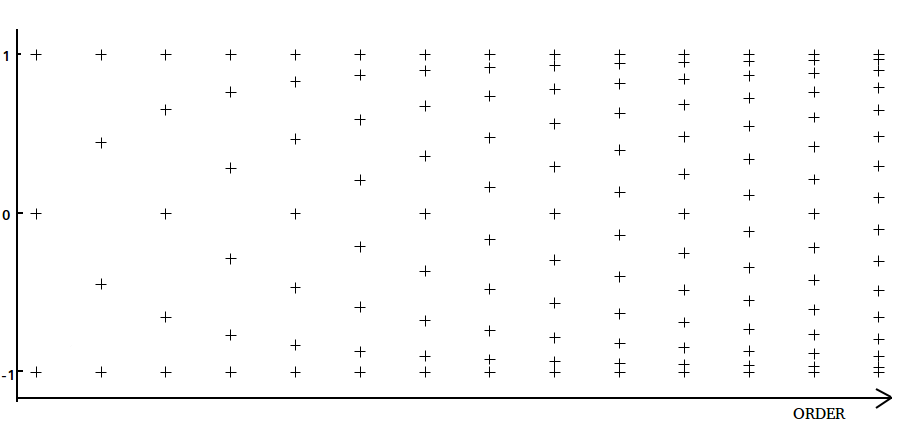
\includegraphics[width=10cm]{gauss-lobatto_points.png}
\caption{\label{GL-points} Gauss-Lobatto points for order $p=2,\dots ,15$.}
\end{figure}

\begin{figure}[h]
\centering
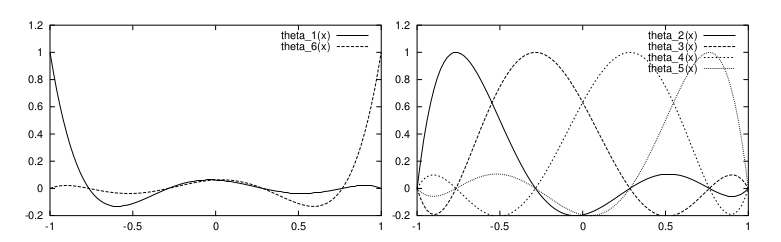
\includegraphics[width=11.5cm]{Gauss-Lobatto-Lagrange_poly.png}
\caption{\label{GLL-poly} Fifth order Gauss-Lobatto-Lagrange polynomials.}
\end{figure}


The continuous Galerkin scheme is applied, implying that, globally, for two contiguous elements $k$ and $k+1$, the polynomial $\theta_p$ in the element $k$ and the polynomial $\theta_0$ in element $k+1$, are considered as one function. This function, known as vertex function and defined in $[0,L]$, is zero in all the domain except in the element $k$ where it takes the values of $\theta_p$ and in element $k+1$ where it takes the values of $\theta_0$. On the other hand we have the bubble functions, that are defined as zero in all the domain except for on element, where they take the value of one of the polynomials $\theta_1$ to $\theta_{p-1}$. Both vertex and bubble functions are shown in Figure \ref{fig-func}.

\begin{figure}[H]
\centering
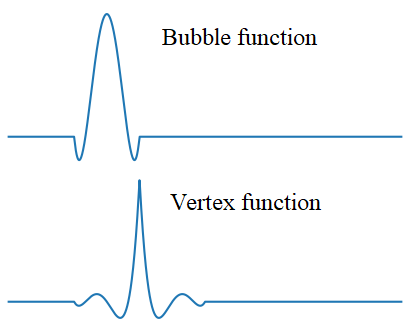
\includegraphics[width=5.5cm]{funciones_globales.png}
\caption{\label{fig-func} Descriptive scheme of vertex and bubble functions.}
\end{figure}

The set of all vertex and bubble functions compose the chosen base. For example for the case of three elements of order three, in Figure \ref{fig-ejemplofunc} all the base functions are shown. There are two special vertex functions, $\phi_0$ and $\phi_{N-1}$, they are only half of the usual vertex functions. In fact, they do not belong to the space of functions $V$, as they are not zero at $s=0$ and $s=L$. This only affects the first and last equations of the system, where the term $\mathbf{\Gamma}$ that does not vanish in the integration by parts must be added, this term is: 

\begin{equation}
\displaystyle
\mathbf{\Gamma} = \left(\ba{c} -\mathbf{F}_0 \\ 0 \\ \vdots\\ 0 \\ \mathbf{F}_{N-1}\\ \ea\right)
\end{equation}

In summary and adding some notation, this are the important aspects of the spatial discretization:

\begin{itemize}
    \item $p$ is the order of the polynomials.
    \item $n-1$ is the number of elements and $h = \frac{L}{m-1}$ is the length of each element.
    \item $N = n + (n-1)(p-1) = p(n-1) + 1$ is the number of base functions\footnote{Note that $n$ is the number of vertex functions and $(n-1)(p-1)$ is the number of bubble functions.}.
    \item $s_i = h\left( \frac{i-(i\%p)}{p} + \frac{1 + \xi_{(i \% p)}}{2} \right)$ are the discretization nodes\footnote{Here $(a\% b)$ denotes the $(a \mod b)$, and the reader should note that $\frac{i-(i\%p)}{p}$ is the element index and $\frac{1 + \xi_{(i \% p)}}{2}$ maps the quadrature nodes from $[-1,1]$ to $[0,1]$.}.
\end{itemize}

\begin{figure}[H]
	\centering
	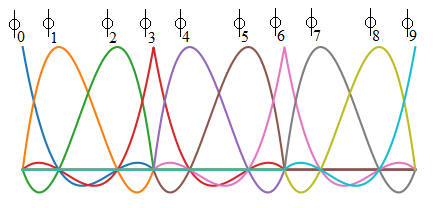
\includegraphics[width=10cm]{notation1.png}
	\caption{\label{fig-ejemplofunc} Example of base functions for three third order elements.}
\end{figure}


For the base choice, the formal formulation would be as follows.

$$\phi_i(s) = \left\{ \ba{l} 
\alpha_i(s) \quad\quad if \quad (i\% p) = 0\quad\\ 
\beta_i(s) \quad\quad else
\ea \right.$$

\vspace{1cm}

where $\alpha_i(s)$ is the vertex function:

$$\alpha_i(s) = \left\{ \ba{l}
\left\{ \ba{l}
\theta_0(2\cdot\frac{s-s_i}{h}-1)\quad if\quad s_{i}\leq s\leq s_{i+p} \\
0\qquad else \\
\ea \right\}\quad if\quad i=0 \\
\\
\left\{ \ba{l}
\theta_p(2\cdot\frac{s-s_{i-p}}{h}-1)\qquad if\quad s_{i-p}\leq s<s_{i} \\
0\qquad else \\
\ea \right\}\quad if\quad i=N-1 \\
\\
\left\{ \ba{l}
\theta_0(2\cdot\frac{s-s_{i}}{h}-1)\quad\quad if\quad s_{i}\leq s\leq s_{i+p}  \\
\theta_p(2\cdot\frac{s-s_{i-p}}{h}-1)\quad\quad if\quad s_{i-p}\leq s<s_{i}  \\
0\quad\quad else \\
\ea \right\}\quad else \\
\ea \right.$$

\vspace{1cm}

and $\beta_i(s)$ is the bubble function:

$$\beta_i(s) = \left\{ \ba{l} 
\theta_{(i\% p)}(2\cdot\frac{s-s_{p(k-1)}}{h}-1)\quad\quad if\quad s_{p\cdot k}\leq s\leq s_{p\cdot (k+1)} \\
0\quad\quad else\\
\ea \right.$$

where $k = \frac{i-(i\%p)}{p}$ is the element index. The base functions are continuous, but their derivatives are not, because of this it is necessary to take a special care when computing derivatives using these functions, and that is done in the next section.\\

\subsubsection{Derivatives and non-linear terms}

With the current basis, if the positions of the discretization nodes, $(r_0, r_1, \dots, r_{N-1})^T$, are known, the derivatives at any point of the chain can be computed with:

$$\frac{\pa^n\mathbf{r}}{\pa s^s}(s)=\sum_{i=0}^{N-1} r_i \frac{\pa^n\phi_i}{\pa s^n}(s)= \left( \frac{\pa^n\phi_0}{\pa s^n}(s), \frac{\pa^n\phi_1}{\pa s^n}(s), \dots , \frac{\pa^n\phi_{N-1}}{\pa s^n}(s) \right)\cdot \left(\ba{c} r_0 \\ r_1 \\ \vdots \\ r_{N-1} \ea\right)$$

In general, it is interesting to compute the derivatives at the discretization nodes, in matrix notation, this can be done with the following expression:

$$\displaystyle
 \left(\ba{c} \frac{\pa^n\mathbf{r}}{\pa s^n}(s_0) \\ \frac{\pa^n\mathbf{r}}{\pa s^n}(s_1) \\ \vdots \\ \frac{\pa^n\mathbf{r}}{\pa s^n}(s_{N-1}) \ea\right) =  \mathbf{D}_n \left(\ba{c} r_0 \\ r_1 \\ \vdots \\ r_{N-1} \ea\right)$$
 
where:

$$\displaystyle
\mathbf{D}_n = \left(\ba{c} \frac{\pa^n\phi_0}{\pa s^n}(s_0)\quad\quad \frac{\pa^n\phi_1}{\pa s^n}(s_0)\quad \dots \quad \frac{\pa^n\phi_{N-1}}{\pa s^n}(s_0) \\ \frac{\pa^n\phi_0}{\pa s^n}(s_1)\quad\quad \frac{\pa^n\phi_1}{\pa s^n}(s_1)\quad \dots\quad \frac{\pa^n\phi_{N-1}}{\pa s^n}(s_0) \\ \vdots\quad\quad\quad\quad\quad\quad\vdots\quad\quad\quad\quad\quad\quad\vdots\\ \frac{\pa^n\phi_0}{\pa s^n}(s_{N-1})\quad \frac{\pa^n\phi_1}{\pa s^n}(s_{N-1}) \dots \frac{\pa^n\phi_{N-1}}{\pa s^n}(s_{N-1}) \ea\right)$$

and for the points where there is a discontinuity in the derivative, the following approximation is used:

$$\displaystyle
\frac{\pa^n\phi_i}{\pa s^n}(s_j) = \frac{1}{2}\left(\frac{\pa^n\phi_i}{\pa s^n}(s_j^{-}) + \frac{\pa^n\phi_i}{\pa s^n}(s_j^{+}) \right)$$

The global derivation matrix of order $n$, $\mathbf{D}_n$ is constant in time and it is computed only once, unless the line length changes, in which case the matrix can be updated with a scalar multiplication. It can be assembled using the local derivation matrix, $\mathbf{D}_n^L$, defined as $(\mathbf{D}_n^L)_{ij}= \frac{\pa^n\theta_j}{\pa x^n}(\xi_i)$, using the following algorithm.

$$\ba{l}
\mathbf{D}_n = \mathbf{0}_{N\times N} \\
\quad \\
for \quad (k=0:n-1)\{ \\
\quad \mathbf{D}_n[ k\cdot p:(k+1)\cdot p,\quad k\cdot p:(k+1)\cdot p ] = \mathbf{D}_n[ k\cdot p:(k+1)\cdot p,\quad k\cdot p:(k+1)\cdot p ] + \mathbf{D}_n^L \\
\} \\
\quad \\
for \quad (k=1:n-1)\{ \\
\quad \mathbf{D}_n[ k\cdot p:(k+1)\cdot p,\quad : \quad ] = \mathbf{D}_n[ k\cdot p:(k+1)\cdot p,\quad : \quad ] \cdot \frac{1}{2} \\
\} \\
\\
\mathbf{D}_n = \left(\frac{2}{l}\right)^n \cdot \mathbf{D}_n
\ea$$

In this algorithm, first the global derivation matrix is initialized and then the values of the local derivation matrix are inserted in the global matrix with a first loop over all elements, as shown in Figure \ref{fig-assemble} for a case with four elements of order three. In a second loop, the rows of the matrix that relate to nodes where the base functions derivatives present discontinuities are divided by two, as shown in Figure \ref{fig-dividebytwo} (the values of the derivatives at both sides of the node were already summed in the previous loop). Finally, the full matrix is multiplied by the factor $\left(\frac{2}{l}\right)^n$, that is necessary because the chain rule of derivation is being applied with the mapping from $[-1,1]$ to $[s_k,s_{k+1}]$ at every element $k$.

\begin{figure}[H]
	\centering
	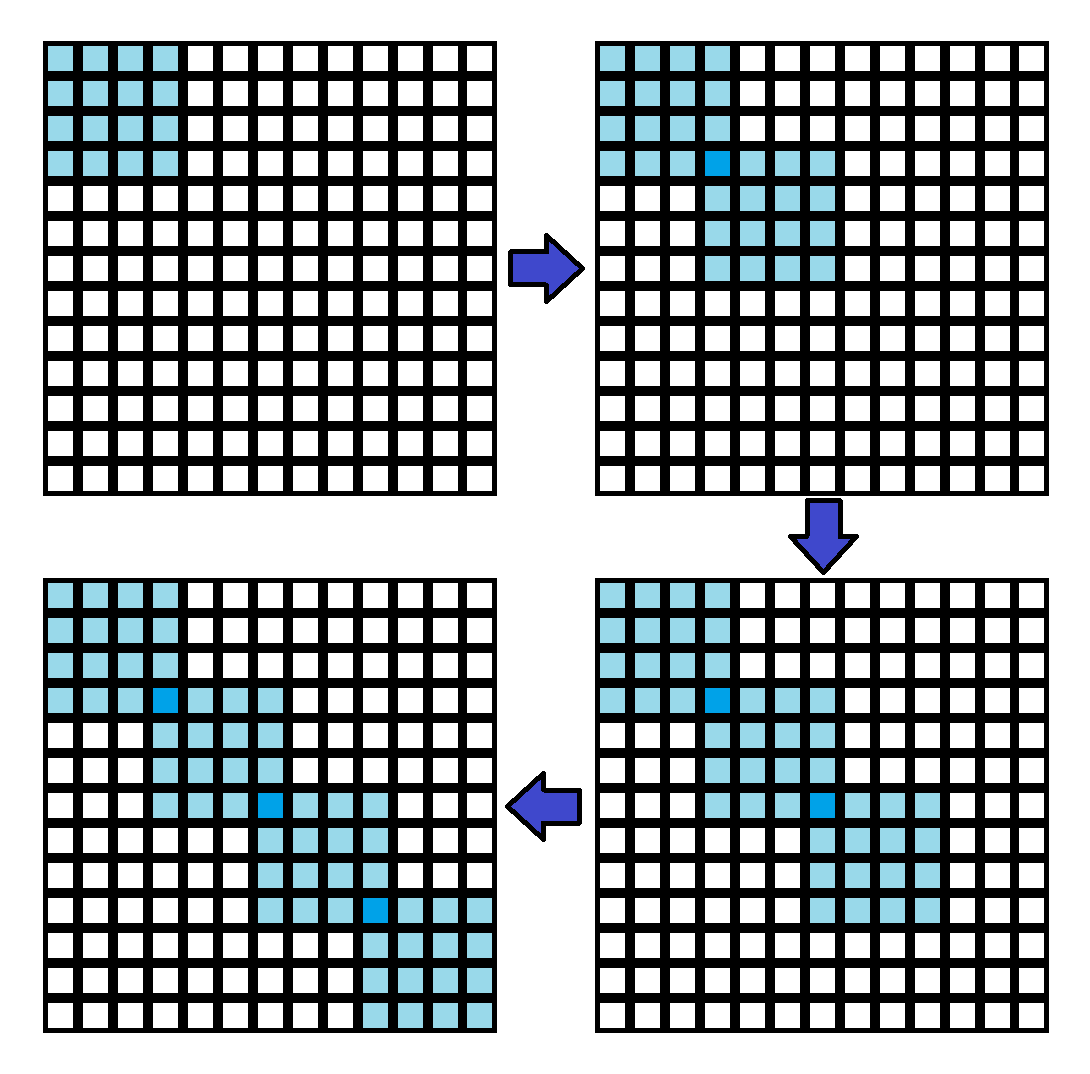
\includegraphics[width=8cm]{1_mat_MK.png}
	\caption{\label{fig-assemble} Assembling step. In the top left corner of the figure, only the first local matrix $\mathbf{D}_n^L$ has been added to the full matrix. In the dark blue elements, the values of $\mathbf{D}_n^L[0,0]$ and $\mathbf{D}_n^L[p,p]$ are being summed. }
\end{figure}

\begin{figure}[H]
	\centering
	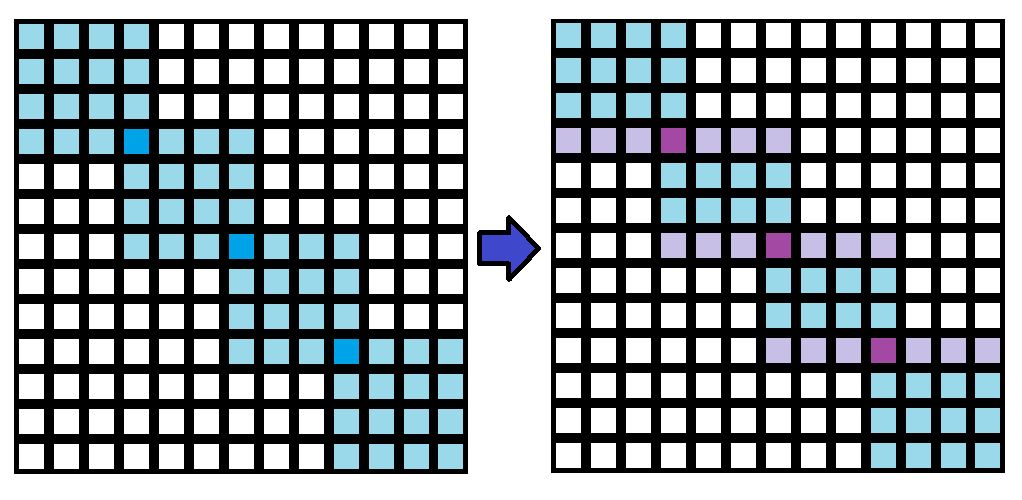
\includegraphics[width=8cm]{1_mat_D.png}
	\caption{\label{fig-dividebytwo} Discontinuity of derivatives treatment. The purple rows are divided by two to average the value of the derivative at both sides of de node.}
\end{figure}

If the line nodes velocities are known, the crossed derivatives at the nodes can also be computed easily using the global derivation matrix:

$$\left(\ba{c} \frac{\pa^n\mathbf{r}}{\pa s^n \pa t}(s_0) \\ \frac{\pa^n\mathbf{r}}{\pa s^n \pa t}(s_1) \\ \vdots \\ \frac{\pa^n\mathbf{r}}{\pa s^n \pa t}(s_{N-1}) \ea\right) =  \mathbf{D}_n \left(\ba{c} \frac{\pa r_0}{\pa t} \\ \frac{\pa r_1}{\pa t} \\ \vdots \\ \frac{\pa r_{N-1}}{\pa t} \ea\right)$$

Once all the derivatives are known, it is easy to compute all the non-linear terms that appear in the expressions of $\mathbf{F}$ and $\hat{\mathbf{f}}$:

\begin{itemize}
	\item $\mathbf{t}(s_i)=\frac{\mathbf{r}'(s_i)}{\left| \mathbf{r}'(s_i) \right|}$
    \item $e(s_i) = |\mathbf{r}'(s_i)| - 1$
    \item $\dot{e}(s_i) = \mathbf{t}(s_i)\cdot\dot{\mathbf{r}}'(s_i)$
\end{itemize}

Although directly computing second or higher order spatial derivatives is possible with this method, the error increases drastically when this is done, and it should always be avoided. For example, in this case, using the weak formulation and integration by parts, it was possible to change a product of a second order derivative with a function for a product of two first order derivatives.

Introducing first order derivatives, which also have a small error, in non-linear expressions where parameters of order up to $10^8$ appear, may produce an error that affects significantly the solution, specially when the interpolated functions are not smooth. \textbf{\textcolor{Red}{For this reason, it would be interesting to perform an analysis of the error, in order to know which is the roughest discretization required to obtain a reasonable solution.}}

\subsubsection{Integrals and system matrices}

In general, for a continuous function $f(x)$ defined in $[-1,1]$, Gauss-Lobatto quadrature of order $p$ can be applied to compute the integral:

$$\int_{-1}^{1} f(x) dx = \sum_{i=0}^{p}\omega_i\cdot f(\xi_{i,p-1}) + E$$

where $E$ is the error of the quadrature rule and the Gauss-Lobatto weights $\{\omega_i\}$ and nodes $\{\xi_{i,p-1}\}$ can be computed with the method detailed in Karniadakis \cite{karniadakis} book, page 61. If $f(x)$ is a polynomial of order less or equal to $2\cdot p-1$, then the quadrature is exact ($E=0$).\\

If a discretization of order $p$ is chosen for the studied line, a quadrature rule of order at least $p+1$ is necessary to evaluate exactly\footnote{If the order of the discretization is $p$, the order of the product $\phi_i\phi_j$ is $2\cdot p$, and a quadrature of order $p$ would be insufficient to compute the integral of this product exactly.} the integrals that appear in Equation \ref{matrices-integrals}. In each element of the discretization, the same local function base is used, and then, the elementary matrices can be used to assemble the full matrices. For element $k$:

$$\mathbf{M}_{ij}^{(k)} = \int_{s_{p\cdot k}}^{s_{p\cdot (k+1)}} \theta_i(\frac{2}{h}(s-s_{p\cdot k})-1) \cdot\theta_j(\frac{2}{h}(s-s_{p\cdot k})-1)ds = \left(\frac{h}{2}\right)\cdot\int_{-1}^{1} \theta_i(x)\cdot\theta_j(x) dx $$

$$\ba{r} \mathbf{K}_{ij}^{*(k)} = \int_{s_{p\cdot k}}^{s_{p\cdot (k+1)}} \left(\theta_i(\frac{2}{h}(s-s_{p\cdot k})-1)\right) ' \cdot\theta_j(\frac{2}{h}(s-s_{p\cdot k})-1)ds = \\
\\
=\int_{s_{p\cdot k}}^{s_{p\cdot (k+1)}} \left(\frac{2}{h}\right)\cdot\theta_i'(\frac{2}{h}(s-s_{p\cdot k})-1) \cdot\theta_j(\frac{2}{h}(s-s_{p\cdot k})-1)ds = \\
\\
=\left(\frac{h}{2}\right)\cdot\int_{-1}^{1} \left(\frac{2}{h}\right)\cdot\theta_i'(x)\cdot\theta_j(x) dx = \int_{-1}^{1} \theta_i'(x)\cdot\theta_j(x) dx \ea$$


These elementary matrices are the same for every element, we define constant elementary matrices $\mathbf{M}^{(e)}$ and $\mathbf{K}^{*(e)}$ as $\mathbf{M}_{ij}^{(e)} = \left(\frac{h}{2}\right)\cdot\int_{-1}^{1} \theta_i(x)\cdot\theta_j(x) dx$ and $\mathbf{K}_{ij}^{*(e)} = \int_{-1}^{1} \theta_i'(x)\cdot\theta_j(x) dx$. The following algorithm is used for assembling of the full matrices:

$$
\ba{l}
\mathbf{M} = \mathbf{0}_{N\times N} \\
\mathbf{K}^* = \mathbf{0}_{N\times N} \\
\quad \\
for \quad (k=0:n-2)\{ \\
\quad \mathbf{M}[ k\cdot p:(k+1)\cdot p+1,\quad k\cdot p:(k+1)\cdot p+1 ] =  \\
\quad \quad \quad =\mathbf{M}[ k\cdot p:(k+1)\cdot p+1,\quad k\cdot p:(k+1)\cdot p+1 ] + \mathbf{M}^{(e)} \\
\quad \mathbf{K}^*[ k\cdot p:(k+1)\cdot p+1,\quad k\cdot p:(k+1)\cdot p+1 ] =  \\
\quad \quad \quad =\mathbf{K}^*[ k\cdot p:(k+1)\cdot p+1,\quad k\cdot p:(k+1)\cdot p+1 ] + \mathbf{K}^{*(e)} \\
\} \\
\ea
$$

This algorithm is the same as the one used for the derivation matrix in Figure \ref{fig-assemble}, but without dividing by two, since there are no discontinuities in this case. Also, the elementary matrices are computed using Gauss-Lobatto Gaussian quadrature with the following algorithm:

$$
\ba{l}
\mathbf{M}^{(e)} = \mathbf{0}_{N\times N} \\
\mathbf{K}^{*(e)} = \mathbf{0}_{N\times N} \\
for \quad (i=0:p)\{ \\
\quad for \quad (j=0:p)\{ \\
\quad \quad for \quad (k=0:p+1)\{ \\
\quad \quad \quad \mathbf{M}^{(e)}[i,j] = \mathbf{M}^{(e)}[i,j] +  \left(\frac{h}{2}\right)\cdot\omega_k\cdot\theta_i(\xi_{k,p})\cdot\theta_j(\xi_{k,p})\\
\quad \quad \quad \mathbf{K}^{*(e)}[i,j] = \mathbf{K}^{*(e)}[i,j] +  \omega_k\cdot\theta'_i(\xi_{k,p})\cdot\theta_j(\xi_{k,p})\\
\quad \quad \} \\
\quad \} \\
\} \\
\ea
$$

In this algorithm there are three nested loops, the first one over the matrix rows, the second one over the matrix columns and the last one is over the quadrature nodes. The system matrices are constant in time and they are computed only once, unless for the matrix $\mathbf{M}$, and only if the line length changes, in which case the matrix can be updated with a scalar multiplication.\\

Recall that the purpose of this whole section was to compute a matrix $\mathbf{A}$ and a vector $\mathbf{B}$ such that:

$$\left(\ba{c} \mathbf{v} \\ \mathbf{a} \ea\right) = \frac{\pa\mathbf{u}}{\pa t} = f(\mathbf{u}, t) = f(\left(\ba{c} \mathbf{r} \\ \mathbf{v} \ea\right), t) = \left(\ba{c} \mathbf{v} \\ \mathbf{A}^{-1}\cdot\mathbf{B} \ea\right)$$

So far, the result is$$\mathbf{A} = \mathbf{M}$$and$$\mathbf{B} = -\mathbf{K}^*\cdot\mathbf{F}+\mathbf{M}\cdot\hat{\mathbf{f}}+\mathbf{\Gamma}$$

where the terms $\mathbf{M}$, $\mathbf{K}^*$, $\mathbf{F}$ and $\hat{\mathbf{f}}$ have been described in detail.\\ \\

Note that the final expression for computing the acceleration at the nodes of the chain is the system $\mathbf{M} \cdot \mathbf{a} =-\mathbf{K}^*\cdot\mathbf{F}+\mathbf{M}\cdot\hat{\mathbf{f}}(\mathbf{a})+\mathbf{\Gamma}$, where $\hat{\mathbf{f}}$ depends on $\mathbf{a}$ because the added mass forces are part of the external force. This problem is solved using an iterative method where the following algorithm is followed, where "tol" is the tolerance of the iterative method and "nIterMax" is the maximum number of iterations, introduced to limit the computational cost.

\begin{equation}
\nonumber
\ba{l} \text{set }\mathbf{a}^0\text{ as the acceleration at previous time-step}\\
\text{solve   }\mathbf{M} \cdot \mathbf{a}^{1} =-\mathbf{K}^*\cdot\mathbf{F}+\mathbf{M}\cdot\hat{\mathbf{f}}(\mathbf{a}^{0})+\mathbf{\Gamma}\\
k = 1\\
\\
while \quad ((||a^{k}-a^{k-1}||>\text{tol})\text{  \&  }(k<\text{nIterMax}))\{ \\
\quad \text{solve   }\mathbf{M} \cdot \mathbf{a}^{k+1} =-\mathbf{K}^*\cdot\mathbf{F}+\mathbf{M}\cdot\hat{\mathbf{f}}(\mathbf{a}^{k})+\mathbf{\Gamma}\\
\quad k = k + 1\\
\}\\
\mathbf{a} = \mathbf{a}^{k}\\
\ea 
\end{equation}

The problem is not completely solved yet. First, it is necessary to describe how to impose the boundary conditions and the initial condition. This is done in the following section.

\subsection{Boundary conditions}

Once the matrix $\mathbf{A}$ and the vector $\mathbf{B}$ in Equation \ref{system-function} are computed, it is necessary to modify them before solving the linear system in order to impose the boundary conditions. In this section, it is shown how to do this for the different options considered.

\subsubsection{Anchor, fairlead or actuator conditions}

When the line is connected to an anchor, a floating body fairlead or a lab actuator, the position, velocity and acceleration of that point of the line are known, and must be imposed. To do so, for computing the internal and external forces vectors, which depend on the position and the velocity of the line, the boundary data is considered in the calculations. Then, before solving the system, first row, last row or both rows of the system matrix are set to zero, except for the element in the diagonal, and in the forces vector the first row, the last row or both rows are changed to the acceleration that the boundary condition imposes. This is shown in Figure \ref{fig-BC1} for a case with four elements of order three where the movements of the line are both of its ends are imposed.

\begin{figure}[H]
	\centering
	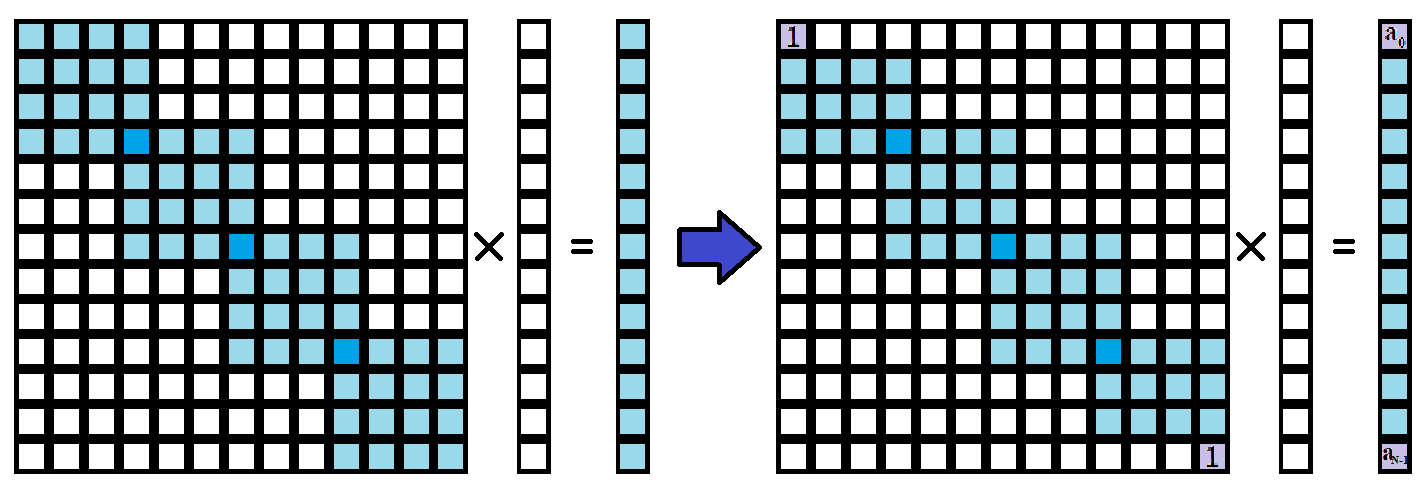
\includegraphics[width=14cm]{BoundaryConditions.png}
	\caption{\label{fig-BC1} Boundary conditions modifications on the system.}
\end{figure}

Formally, this changes are expressed with the following pseudo-code:

\begin{equation}
\nonumber
\ba{l} \mathbf{A} = \mathbf{M}\\
\mathbf{A}[0,0] = 1\\
\mathbf{A}[0,1:N-1] = 0\\
\mathbf{A}[N-1,N-1] = 1\\
\mathbf{A}[N-1,0:N-2] = 0\\
\\
\mathbf{B} = -\mathbf{K}^*\cdot\mathbf{F}+\mathbf{M}\cdot\hat{\mathbf{f}}+\mathbf{\Gamma}\\
\mathbf{B}[0,:] = \hat{\mathbf{a}}_0\\
\mathbf{B}[N-1,:] = \hat{\mathbf{a}}_{N-1}\\
\ea 
\end{equation}

where $\hat{\mathbf{a}}_0$ and $\hat{\mathbf{a}}_{N-1}$ are the accelerations imposed at nodes $0$ and $N-1$ respectively.\\


\subsubsection{Multi-line joint conditions}

An important feature of a line simulation software is to be able study the case where more than one line are connected to one point. An example of this situation is the crowfoot or delta mooring system, where there are two fairleads, one anchor, and three lines that join these three points to a common one, as shown in Figure \ref{fig-crowfoot}.

\begin{figure}[H]
	\centering
	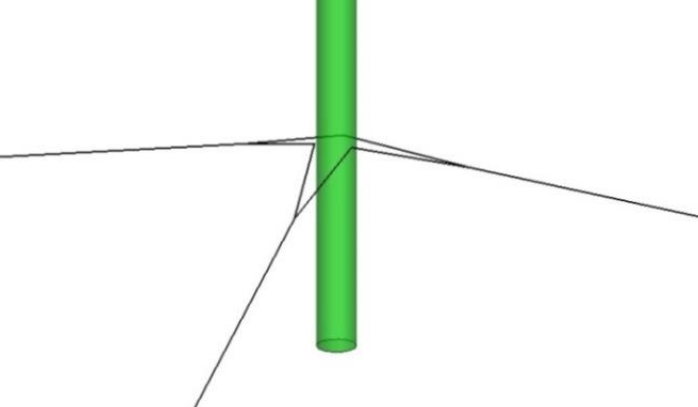
\includegraphics[width=8cm]{crowfoot.PNG}
	\caption{\label{fig-crowfoot} Crowfoot or delta mooring system.}
\end{figure}

Let there be a set of $n$ lines converging to the same point, where $\{(\rho_0)_i\}$ are the linear weights of the different lines. In order to apply the joint boundary condition, first, the averages of the positions and the velocities of all the nodes that converge to the joint are imposed to those nodes, before computing the internal and external forces vectors. After that, the lines systems are solved without making any change to the equations of the nodes that are connected to the joint. Then, once the accelerations of all the nodes connected to the joint, $\{\hat{\mathbf{a}}_i\}$, are known, the acceleration of the joint, $\mathbf{a}_J$ is computed as:

$$\mathbf{a}_J = \frac{\sum_{i = 1}^n\left[(\rho_0)_i\cdot\hat{\mathbf{a}}_i\right]}{\sum_{i = 1}^n(\rho_0)_i}$$

Finally, this acceleration is imposed to all the nodes that converge to the joint.

\subsubsection{Winch condition}

Other important feature is to be able to simulate lines connected to winches, that may vary their length depending on the momentum applied with the winches engines, $M$, the properties of the winches (radius $R$ and mass $m$) and the tension $T$ of the lines at the winches. Figure \ref{fig-winche} shows the scheme of a winch.\\

\begin{figure}[H]
	\centering
	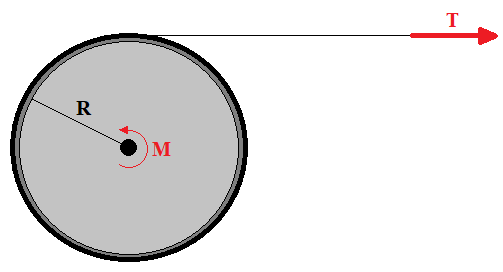
\includegraphics[width=8cm]{winch.PNG}
	\caption{\label{fig-winche} Winch scheme.}
\end{figure}

\vspace{1cm}

There are two aspects that we have to consider when there is a winch at the end of a line. The first one is how to compute how the winch rotates, and the second one is to compute how the winch rotation modifies the line length, and how the length variation affects the equations of the line.

In order to simulate the rotation of the winch, the Newton equation is applied in Equation \ref{eq-winch}.

\bean I\cdot \alpha = T\cdot r - M \label{eq-winch}\eean

The left side of Equation \ref{eq-winch} is the product of moment of inertia of the winch with the angular acceleration of the winch for rotations around the winch's axis. If the winch is considered to be a cylinder, the moment of inertia of the winch is $I=\frac{1}{2}\cdot m\cdot R^2$. The right side of the equation is the sum of the momentum that is applied to the winch, first the momentum that the line applies, considering that the radius of the winch and the tension of the line are perpendicular, and finally the momentum that the winch's engine applies. The signs are chosen some how that if the angle of rotation of the winch is positive, the line length increases, and if the winch's engine applies a positive momentum strong enough, the line length decreases.

Winch's time evolution is then described by the following initial value problem:

$$\left\{ \ba{l} \frac{\pa\mathbf{u}}{\pa t} = f(t) \\  \\ \mathbf{u}(0) = \mathbf{u}_0 \ea \right.$$

With $f$ being the ODE function, $\mathbf{u}_0$ known initial condition, and $\mathbf{u}$ the unknown. In this case the unknown will be: 

$$\mathbf{u}=\left(\ba{c} \theta \\ \omega \ea\right) $$

where $\theta$ and $\omega$ are, respectively, the rotation and the angular velocity of the winch. The initial condition will be considered as zero:

$$\mathbf{u}_0=\left(\ba{c} 0 \\ 0 \ea\right) $$

and the ODE function is:

\bean
\left(\ba{c} \omega \\ \alpha \ea\right) = \frac{\pa\mathbf{u}}{\pa t} = f(t) = \left(\ba{c} \omega \\ I^{-1}\cdot(T\cdot r - M) \ea\right)
\label{system-function-winch}
\eean

This ODE is integrated together with the line ODE, and the coupling between the winch and the line consists in that the line tension is used in the winch ODE and the winch rotation is used un the line ODE. This is because the line length is dependent on the winch rotation as it is shown in Equation \ref{eq-winchL}.

\bean L = L_0 + \theta\cdot R \label{eq-winchL}\eean

where $L$ is the line length, $L_0$ is the initial line length, and $theta$ and $R$, are respectively and as mentioned before, the winch rotation and radius. When the line length changes, instead of using the global derivation matrices $\mathbf{D}_n$ and the mass matrix $\mathbf{M}$ described in the previous section and used in the line ODE, the following matrices must be used instead:

$$\mathbf{D}_n \Rightarrow \left(\frac{L_0}{L}\right)^n\cdot\mathbf{D}_n$$
$$\mathbf{M} \Rightarrow \left(\frac{L}{L_0}\right)\cdot\mathbf{M}$$

With this, all the studied boundary conditions are already described, and only the last step is needed: the computation of the initial condition for all the line nodes.

\vspace{1cm}

\subsection{Initial condition}

For the initial condition, in general, a quasi-static (QS) method is used to find the positions of the line nodes. The velocity and acceleration of these nodes are considered as zero for the initial conditions. The QS method used is based in \cite{faltinsen}, an in this section a description of the method is presented. \\ \\

The QS method ignores the dynamic effects on the line as inertia, friction, damping, or added mass and considers the line to be contained in a plane. The variables used for the QS method are:\\ \\

\begin{tabular}{ll}
	$\rho_w$ & water density, \\ 
	$A$ & line section \\
	$\rho_0$ & line mass per unit of length, \\
	$\mathbf{g}$ & gravity acceleration vector, \\
	$x_{F}$ & horizontal span between line ends, \\
	$z_{F}$ & vertical span between line ends, \\
	$H_{F}$ & horizontal tension at line's top support (usually the fairlead), \\
	$V_{F}$ & vertical tension at line's top support, \\
	$H_{A}$ & horizontal tension at line's bottom support (usually the anchor), \\
	$V_{A}$ & vertical tension at line's bottom support, \\
	$\omega = (\rho_0-rho_w\cdot A)*g$ & line's underwater weight, \\
	$L$ & line length, \\
	$L_B$ & line length lying over the sea floor, \\
	$E$ & line Young's modulus and \\
	$C_{B}$ & line-ground friction coefficient. \\ \\
\end{tabular}

Usually, the horizontal and vertical spans $x_{F}$ and $z_{F}$ are known and the unknowns are the tension values at both ends of the line. 

\vspace{1cm}
On literature, the following expressions are found for the horizontal an vertical spans in terms of the top support tension:\\

\hspace{1cm}\textbf{If the line does not lie on the sea floor} ($L_B = L - \frac{V_F}{\omega} \leq 0$):

\begin{equation}
\nonumber
x(H_{F},V_{F}) = \frac{H_{F}}{\om} \left[ \ln \left( \frac{V_{F}}{H_{F}} + \sqrt{1+\left( \frac{V_{F}}{H_{F}} \right)^{2} } \right) - \ln \left( \frac{V_{F}-\om L}{H_{F}} + \sqrt{1+\left( \frac{V_{F}-\om L}{H_{F}} \right)^{2} } \right) \right] + \frac{H_{F} L}{EA}
\end{equation}

\begin{equation}
\nonumber
z(H_{F},V_{F}) = \frac{H_{F}}{\om} \left[\sqrt{1+\left( \frac{V_{F}}{H_{F}} \right)^{2} } - \sqrt{1+\left( \frac{V_{F}-\om L}{H_{F}} \right)^{2} } \right] + \frac{1}{EA} \left( V_{F} L - \frac{\om L^{2}}{2}\right)
\end{equation}

\vspace{1cm}
\hspace{1cm}\textbf{If part of the line lies on the sea floor}\footnote{In this case, there is a "max" term, which differentiates if there is horizontal tension in the anchor or not. This should be considered as two separate cases for the Newton-Raphson method in order to compute the Jacobean matrix derivatives.} ($L_B = L - \frac{V_F}{\omega} > 0$):

\begin{multline}
\nonumber
x(H_{F},V_{F}) = L - \frac{V_{F}}{\om} + \frac{H_{F}}{\om} \ln \left( \frac{V_{F}}{H_{F}} + \sqrt{1+\left( \frac{V_{F}}{H_{F}} \right)^{2} } \right)  + \frac{H_{F} L}{EA}+ \\
+ \frac{C_{B} \om}{2 EA} \left[ - \left( L - \frac{V_{F}}{\om} \right)^{2} + \left( L - \frac{V_{F}}{\om}  - \frac{H_{F}}{C_{B}\om}\right) \max \left( L - \frac{V_{F}}{\om} - \frac{H_{F}}{C_{B}\om},0 \right)
\right]
\end{multline}

\begin{equation}
\nonumber
z(H_{F},V_{F}) = \frac{H_{F}}{\om} \left[\sqrt{1+\left( \frac{V_{F}}{H_{F}} \right)^{2} } - 1 \right]
+ \frac{1}{EA} \left( V_{F} L - \frac{\om L^{2}}{2}\right) 
\end{equation}

\vspace{1cm}

Finding the pair $(H_{F},V_{F})$ that yields the desired spans implies solving a non-linear system of equations, and this is done using a Newton-Raphson method. To do so, the function $\mathbf{F}(H_{F},V_{F})$ is the defined as:

$$\mathbf{F}(H_{F},V_{F}) = \left(\ba{c} x(H_{F},V_{F}) - x_{F} \\ z(H_{F},V_{F}) - z_{F} \ea\right)$$

in a way that the solution of the equation $\mathbf{F}(H_{F},V_{F})=0$ is the solution of the non-linear system. Let $\mathbf{J}$ be the Jacobean matrix of $\mathbf{F}$. Let the unknown be expressed as $\mathbf{x} = (H_{F}, V_{F})^T$. Let the initial guess be:

$$ \mathbf{x}^0 = \left(\left| \frac{\om x_{F}}{2 \lambda_{0}}\right|, \frac{\om}{2} \left[\frac{z_{F}}{\tanh(\lambda_{0})} + L \right]\right)^T $$

where:

$$ \lambda_{0} = \left\{ \ba{ll} 
10^{6}                                                 & \text{for } x_{F} = 0 \\ 
0.2                                                    & \text{for } \sqrt{x_{F}^2+z_{F}^2} \geq L \\
\sqrt{3 \left( \frac{L^2-z_{F}^2}{x_{F}^2} - 1 \right)} & \text{otherwise.} \ea \right. $$

Then the solution is obtained updating the estimation of the solution with the expression:

$$\mathbf{x}^{k+1} = \mathbf{x}^{k} - \mathbf{J}^{-1}(\mathbf{x}^{k})\cdot\mathbf{F}(\mathbf{x}^{k})$$

until the convergence criteria $||\mathbf{x}^{k+1} - \mathbf{x}^{k}||< \text{tol}$ is met, where "tol" is the tolerance, or until the maximum number of iterations is reached.


Once the tension at the top support is obtained, the tension at the bottom can be easily computed with:\\

\hspace{1cm}\textbf{If the line does not lie on the sea floor}:

\begin{equation}
\nonumber
H_{A} = H_{F} \qquad V_{A} = V_{F} - \om L
\end{equation}

\vspace{1cm}
\hspace{1cm}\textbf{If part of the line lies on the sea floor}:

\begin{equation}
\nonumber
H_{A} = \max(H_{F} - C_{B} \om L_{B},0) \qquad V_{A} = 0
\end{equation}


\vspace{1cm}

Finally, the position and tension of any point of the line can be computed with the following expressions:


\hspace{1cm}\textbf{If the line does not lie on the sea floor}:

\bean
\nonumber
x(s) = \frac{H_{F}}{\om} \left[ \ln \left( \frac{V_{A} + \om s}{H_{F}} + \sqrt{1+\left( \frac{V_{A}+\om s}{H_{F}} \right)^{2} } \right) - \ln \left( \frac{V_{A}-\om L}{H_{F}} + \sqrt{1+\left( \frac{V_{A}-\om L}{H_{F}} \right)^{2} } \right) \right] + \frac{H_{F} s}{EA} 
\eean

\bean
\nonumber
z(s) = \frac{H_{F}}{\om} \left[\sqrt{1+\left( \frac{V_{A}+\om s}{H_{F}} \right)^{2} } - \sqrt{1+\left( \frac{V_{A}}{H_{F}} \right)^{2} } \right] + \frac{1}{EA} \left( V_{A} s - \frac{\om s^{2}}{2}\right)
\eean

\bean
\nonumber
T_{e}(s) = \sqrt{H_{F}^{2} + (V_{A} + \om s)^{2}}
\eean

\vspace{1cm}
\hspace{1cm}\textbf{If part of the line lies on the sea floor}:

\bean
\nonumber
\hspace{-0.5cm} x(s) =  \left\{ \ba{cl} s, & \hspace{-0.25cm} 0 \leq s \leq L_{B} - \frac{H_{F}}{C_{B} \om} \\ & \\
s + \frac{C_{B} \om}{2EA} \left[ \ba{lr} s^{2} - 2 \left(L_{B} - \frac{H_{F}}{C_{B} \om} \right) s \\+\left(L_{B} - \frac{H_{F}}{C_{B} \om}  \right)  \max\left(L_{B} - \frac{H_{F}}{C_{B} \om} ,0\right) \ea \right] 
, & \hspace{-0.25cm} L_{B} - \frac{H_{F}}{C_{B} \om}   \leq s \leq L_{B}\\ & \\
\ba{lr}L_{B} + \frac{H_{F}}{\om} \ln \left[ \frac{\om(s-L_{B})}{H_{F}} + \sqrt{1+\left(\frac{\om(s-L_{B})}{H_{F}} \right)^{2}} \right] + \frac{H_{F}s}{EA} \\
+ \frac{C_{B} \om}{2EA} \left[ -L_{B}^{2} + \left(L_{B} - \frac{H_{F}}{C_{B} \om}  \right)  \max\left(L_{B} - \frac{H_{F}}{C_{B} \om} ,0\right) \right]\ea 
, & \hspace{-0.25cm} L_{B}   \leq s \leq L
\ea \right.
\eean

\bean
\nonumber
z(s) =  \left\{ \ba{cl} 0, & 0 \leq s \leq L_{B} \\ & \\
\frac{H_{F}}{\om} \left[\sqrt{1+\left( \frac{V_{F}}{H_{F}} \right)^{2} } - 1 \right] + \frac{1}{EA} \left( V_{F} L - \frac{\om L^{2}}{2}\right) , & L_{B}  \leq s \leq L \ea \right.
\eean

\bean
\nonumber
T_{e}(s) = \left\{ \ba{cl} \max(H_{F} + C_{B} \om (s - L_{B}),0), & 0 \leq s \leq L_{B} \\ & \\
\sqrt{H_{F}^{2} + (\om (s-L_{B}))^{2}}, & L_{B}  \leq s \leq L \ea \right.
\eean

This is enough to compute the initial condition for most of the cases, but there are some exceptions in which the iterative method does not converge, or when the line system is not valid for the quasi-static approximation, for example, when there is a crowfoot joint or when the line is too tense. In this cases, an approximated initial condition will be used, considering the lines straight between their ends, and a previous simulation must be done to find the equilibrium state, which will be considered as the initial condition for other simulations.

Also if the case of study does not require a really precise mooring or towing lines simulation, or needs to be really fast, the QS method can be coupled with the floating bodies to run time evolution simulation.

\clearpage
%%%%%%%%%%%%%%%%%%%%%%%%%%%%%%%%%%%%%%%%%%%%%%%%%%%%%%%%%%%%%%%%%%%%%%%%%%%
%   Wind turbine
%%%%%%%%%%%%%%%%%%%%%%%%%%%%%%%%%%%%%%%%%%%%%%%%%%%%%%%%%%%%%%%%%%%%%%%%%%%
\section{Wind turbine}
To be developed.


%%%%%%%%%%%%%%%%%%%%%%%%%%%%%%%%%%%%%%%%%%%%%%%%%%%%%%%%%%%%%%%%%%%%%%%%%%%
%   Oscillating water columns
%%%%%%%%%%%%%%%%%%%%%%%%%%%%%%%%%%%%%%%%%%%%%%%%%%%%%%%%%%%%%%%%%%%%%%%%%%%
\section{Oscillating water columns}
To be developed.


%%%%%%%%%%%%%%%%%%%%%%%%%%%%%%%%%%%%%%%%%%%%%%%%%%%%%%%%%%%%%%%%%%%%%%%%%%%
%   Mechanical systems
%%%%%%%%%%%%%%%%%%%%%%%%%%%%%%%%%%%%%%%%%%%%%%%%%%%%%%%%%%%%%%%%%%%%%%%%%%%
\section{Mechanical systems}
(Alvaro) (6 DOF springs)


%%%%%%%%%%%%%%%%%%%%%%%%%%%%%%%%%%%%%%%%%%%%%%%%%%%%%%%%%%%%%%%%%%%%%%%%%%%
%   Time integration
%%%%%%%%%%%%%%%%%%%%%%%%%%%%%%%%%%%%%%%%%%%%%%%%%%%%%%%%%%%%%%%%%%%%%%%%%%%
\section{Time integration}
(Alvaro) (BDF2 with variable step)


%%%%%%%%%%%%%%%%%%%%%%%%%%%%%%%%%%%%%%%%%%%%%%%%%%%%%%%%%%%%%%%%%%%%%%%%%%%
%   Coupling
%%%%%%%%%%%%%%%%%%%%%%%%%%%%%%%%%%%%%%%%%%%%%%%%%%%%%%%%%%%%%%%%%%%%%%%%%%%
\section{Coupling}
(Alvaro) (Weak coupling)



\clearpage

\bibliographystyle{empty} %%%%%%%%%%%%%%%%%%%%%%%%%%%%%%%%%%%%%%%%%%%%%%%%%%%%%%%%%%%%%%%%%%%%%%%%%%%%%%
\begin{thebibliography}{9}
	
\bibitem{ODEPACK}
A. C. Hindmarsh, ODEPACK, A Systematized Collection of ODE Solver, Editors:Stepleman, Carver, Peskin, Ames and Vichnevetsky: IMACS Transactions on Scientific Computation, 1983.

\bibitem{karniadakis}
G. E. Karniadakis, Spectral/hp Element Methods for computational Fluid Dynamics. Second Edition. Oxford science Publications, 2004.

\bibitem{azcona}
J. Azcona, Computational and Experimental Modelling of Mooring Lines Dynamics for Offshore Floating Wind Turbines. UPM. 2015

\bibitem{ref-drag}
J. N. Newman, Marine Hydrodynamics, The Massachusetts Institute of Technology, 1977

\bibitem{Palm-2017} 
J. Palm, C. Eskilsson and L. Bergdahl. An hp-adaptive discontinuous Galerkin method for modelling snap loads in mooring cables. Ocean Engineering, 144: 266-276, 2017.

\bibitem{Aamo-2000}
O.M. Aamo and T.I. Fossen. Finite element modelling of mooring lines. Mathematics and Computers in Simulation, 53(4-6):415 – 422, 2000.

\bibitem{faltinsen}
O.M. Faltinsen, Sea loads on ships and offshore structures.Cambridge ocean technology series. 1999

\bibitem{Hall-2015}
M. Hall and A. Goupee. Validation of a lumped-mass mooring line model with DeepCwind semisubmersible model test data. Ocean Engineering,104:590 – 603, 2015.

\bibitem{torsion}
M. R. Escalante, M.B. Rosales, R. Sampaio and T. Ritto, Reduced order model of a 3D cable using proper orthogonal decomposition. Mec. Comp.. 30. 1143-1158. 2011

\bibitem{quintela}
P. Est\'evez. Matemáticas en ingeniería con MATLAB (Vol. 3). Universidad de Santiago de Compostela. 2001


\end{thebibliography}


\end{document}